\documentclass[a4paper]{article}


%usepackages
\usepackage{float} % Improves the positioning of figures
\usepackage{amsmath} % Providing numerous mathematical symbols, structures, and...
\usepackage{amssymb} % Typesetting mathematical statements
\usepackage{amsthm} % Typesetting theorems
\usepackage{authblk} % Provides additional block environments
\usepackage{graphicx} % To include external graphics files
\usepackage{caption} % Provides enhanced caption formatting options for figures
\usepackage{xcolor} % Extends the color capabilities
\usepackage{mdframed} % Enables the creation of framed box


\newtheorem{thm}{Theorem} % Define the theorem environment


% Set the background color of theorem
\newmdtheoremenv[
backgroundcolor= gray!30,
hidealllines=true
]{cthm}{Theorem} 


% Title, author, affiliation and date
\title{The slope problem}
\author{Mobina Khaksar}
\affil{K. N. Toosi University of Technology, Faculty of Mathematics, Department of Computer Science}
\date{}


\begin{document}

\maketitle

\newpage
\noindent
Try for yourself — before you read much further — to construct configurations of points in the plane that determine “relatively few” slopes. For this we assume, of course, that the $n \geq 3$ points do not all lie on one line. Recall from Chapter 11 on “Lines in the plane” the theorem of Erd\H{o}s and de ˝ Bruijn: the $n$ points will determine at least $n$ different lines. But of course many of these lines may be parallel, and thus determine the same slope.

\begin{figure}[H]
    \centering
    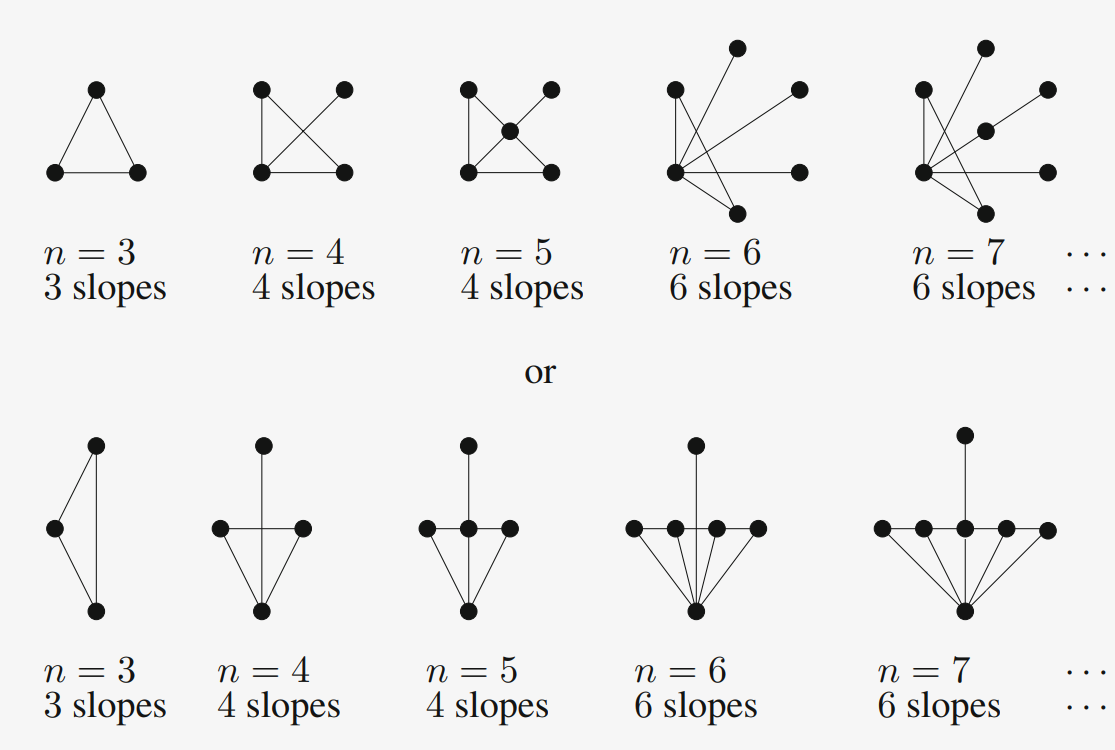
\includegraphics[scale=0.4]{pics/picture1.png}
    \caption{A little experimentation for small $n$ will probably lead you to a sequence such as the two depicted here.}
\end{figure}
    
\noindent
After some attempts at finding configurations with fewer slopes you might conjecture — as Scott did in 1970 — the following theorem.
\begin{cthm}\label{thm1}
If $n \geq 3$ points in the plane do not lie on one single line, then they determine at least $n - 1$ different slopes, where equality is possible only if $n$ is odd and $n \geq 5$.
\end{cthm}

\noindent
Our examples above — the drawings represent the first few configurations in two infinite sequences of examples — show that the theorem as stated is best possible: for any odd $n \geq 5$ there is a configuration with $n$ points that determines exactly $n - 1$ different slopes, and for any other $n \geq 3$ we have a configuration with exactly $n$ slopes.

\noindent
However, the configurations that we have drawn above are by far not the only ones. For example, Jamison and Hill described four infinite families of configurations, each of them consisting of configurations with an odd number $n$ of points that determine only $n - 1$ slopes (slope-critical configurations). Furthermore, they listed 102 sporadic examples that do not seem to fit into an infinite family, most of them found by extensive computer searches.

\noindent
Conventional wisdom might say that extremal problems tend to be very difficult to solve exactly if the extreme configurations are so diverse and irregular. Indeed, there is a lot that can be said about the structure of slopecritical configurations (see [2]), but a classification seems completely out of reach. However, the theorem above has a simple proof, which has two main ingredients: a reduction to an efficient combinatorial model due to Eli Goodman and Ricky Pollack, and a beautiful argument in this model by which Peter Ungar completed the proof in 1982.


\begin{proof}
\textbf{(1)} First we notice that it suffices to show that every “even” set of $n = 2m$ points in the plane $(m \geq 2)$ determines at least $n$ slopes. This is so since the case $n = 3$ is trivial, and for any set of $n = 2m + 1 \geq 5$ points (not all on a line) we can find a subset of $n - 1=2m$ points, not all on a line, which already determines $n - 1$ slopes. 

\noindent
Thus for the following we consider a configuration of $n = 2m$ points in the plane that determines $t \geq 2$ different slopes.


\noindent
\textbf{(2)} The combinatorial model is obtained by constructing a periodic sequence of permutations. For this we start with some direction in the plane that is not one of the configuration’s slopes, and we number the points $1,\ldots,n$ in the order in which they appear in the 1-dimensional projection in this direction. Thus the permutation $\pi_0 = 123 \ldots n$ represents the order of the points for our starting direction.

\noindent
Next let the direction perform a counterclockwise motion, and watch how the projection and its permutation change. Changes in the order of the projected points appear exactly when the direction passes over one of the configuration’s slopes. 

\noindent
But the changes are far from random or arbitrary: By performing a $180^\circ$ rotation of the direction, we obtain a sequence of permutations

\begin{center}
$ \pi_0 \rightarrow \pi_1 \rightarrow \pi_2 \rightarrow \ldots \rightarrow \pi_{t-1} \rightarrow \pi_t $
\end{center}

\noindent
which has the following special properties:

\begin{itemize}
  \item The sequence starts with $\pi_0 = 123 \ldots n$ and ends with $\pi_t = n \ldots 321$.
  \item The length $t$ of the sequence is the number of slopes of the point configuration.
  \item In the course of the sequence, every pair $i < j$ is switched exactly once. This means that on the way from $\pi_0 = 123 \ldots n$ to $\pi_t = n \ldots 321$, only \textit{increasing} substrings are reversed.
  \item Every move consists in the reversal of one or more disjoint increasing substrings (corresponding to the one or more lines that have the direction which we pass at this point).
\end{itemize}

\begin{figure}[H]
    \centering
    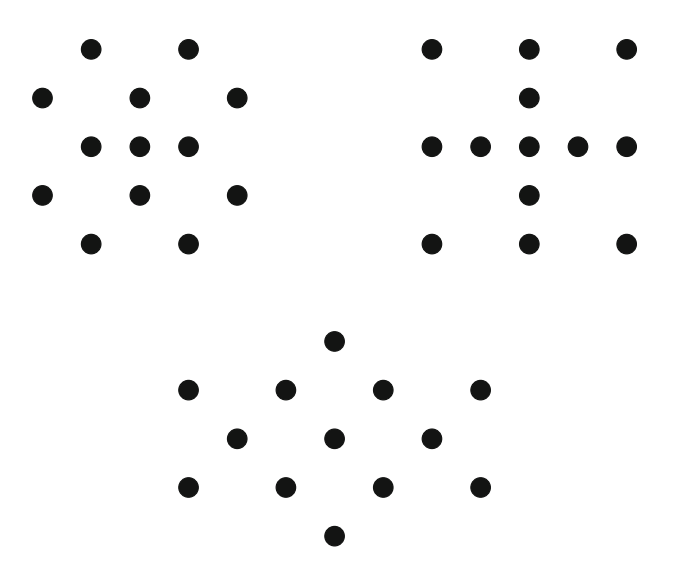
\includegraphics[scale=0.4]{pics/picture2.png}
    \caption{Three pretty sporadic examples from the Jamison–Hill catalogue}
\end{figure}

\begin{figure}[H]
    \centering
    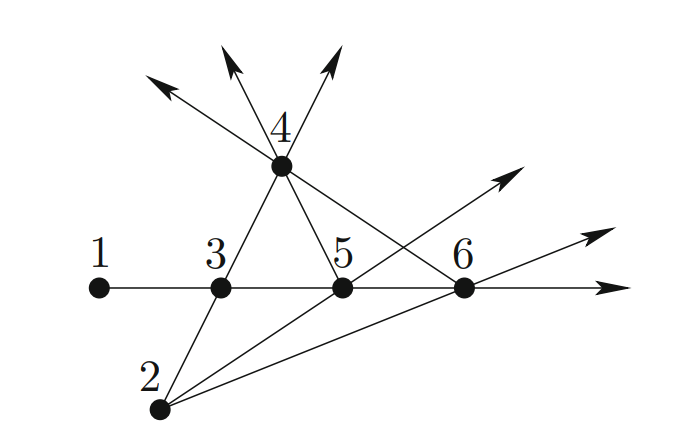
\includegraphics[scale=0.4]{pics/picture3.png}
    \caption{This configuration of $n = 6$ points determines $t = 6$ different slopes.}
\end{figure}

\begin{figure}[H]
    \centering
    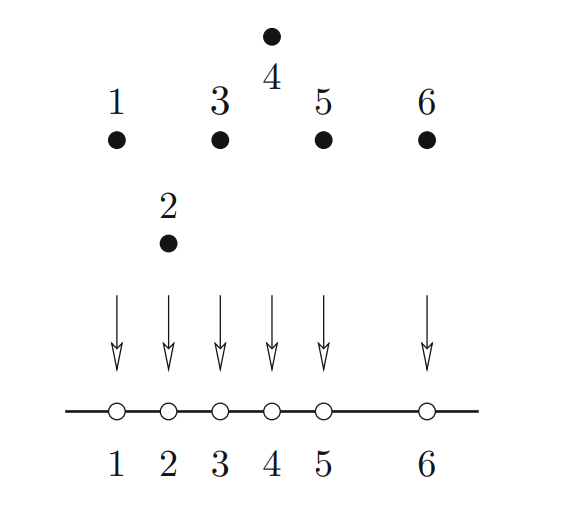
\includegraphics[scale=0.4]{pics/picture4.png}
    \caption{Here a vertical starting direction yields $\pi_0 = 123456$.}
\end{figure}

\begin{figure}[H]
    \centering
    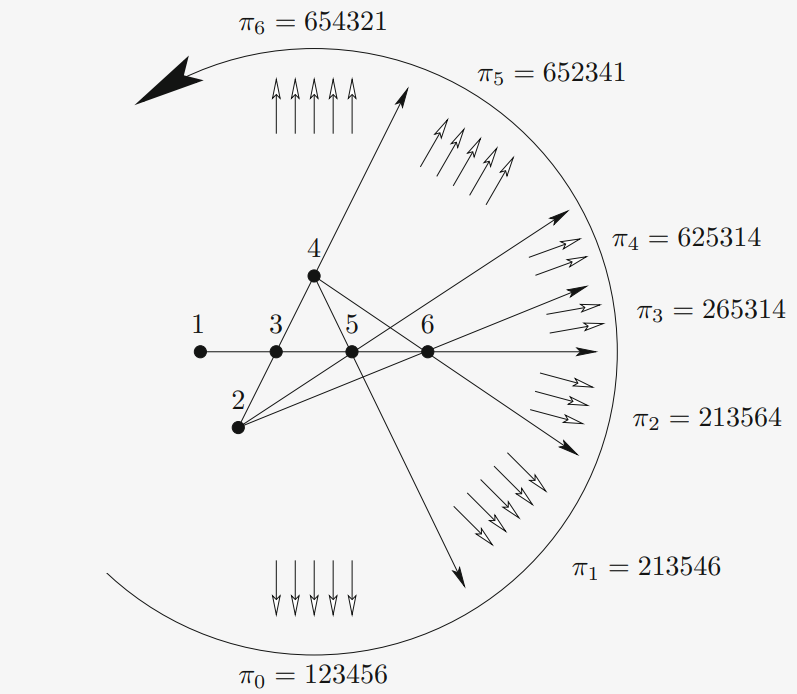
\includegraphics[scale=0.6]{pics/picture5.png}
    \caption{Getting the sequence of permutations for our small example}
\end{figure}

\noindent
By continuing the circular motion around the configuration, one can view the sequence as a part of a two-way infinite, periodic sequence of permutations

\begin{center}
$ \ldots \rightarrow \pi_{-1}  \rightarrow \pi_0 \rightarrow \ldots \rightarrow \pi_t \rightarrow \pi_{t+1} \rightarrow \ldots \rightarrow \pi_{2t} \rightarrow \ldots $
\end{center}

\noindent
where $\pi_{i+t}$ is the reverse of $\pi_i$ for all $i$, and thus $\pi_{i+2t} = \pi_i$ for all $i \in \mathbb{Z}$. We will show that \textit{every} sequence with the above properties (and $t \geq 2$) must have length $t \geq n$.

\noindent
\textbf{(3)} The proof’s key is to divide each permutation into a “left half” and a “right half” of equal size $m = \frac{n}{2}$ , and to count the letters that cross the imaginary \textit{barrier} between the left half and the right half. 

\noindent
Call  $\pi_i \rightarrow \pi_{i+1}$  a \textit{crossing move} if one of the substrings it reverses does involve letters from both sides of the barrier. The crossing move has \textit{order d} if it moves $2d$ letters across the barrier, that is, if the crossing string has exactly $d$ letters on one side and at least $d$ letters on the other side. Thus in our example

\begin{center}
$\pi_2$ = 2\(\underline{13:56}\)4 $\longrightarrow$ 2\(\overline{65:31}\)4 = $\pi_3$ 
\end{center}

\noindent
is a crossing move of order $d = 2$ (it moves 1, 3, 5, 6 across the barrier, which we mark by “:”), 

\begin{center}
65\(\underline{2:34}\)1 $\longrightarrow$ 65\(\overline{4:32}\)1
\end{center}

\noindent
is crossing of order $d = 1$, while for example 

\begin{center}
6\(\underline{25}\):3\(\underline{14}\) $\longrightarrow$ 6\(\overline{52}\):3\(\overline{41}\)
\end{center}

\noindent
is not a crossing move.

\noindent
In the course of the sequence $\pi_0 \rightarrow \pi_1 \rightarrow \ldots \rightarrow \pi_t$, each of the letters $1, 2,\ldots,n$ has to cross the barrier at least once. This implies that, if the orders of the $c$ crossing moves are $d_1, d_2, \ldots, d_c$, then we have

\begin{center}
$\sum_{i=1}^{c} 2d$  = \#\{letters that cross the barrier\} $\geq$ n.
\end{center}

\noindent
This also implies that we have at least two crossing moves, since a crossing move with $2d_i = n$ occurs only if all the points are on one line, i. e. for $t = 1$. Geometrically, a crossing move corresponds to the direction of a line of the configuration that has less than $m$ points on each side.

\begin{figure}[H]
    \centering
    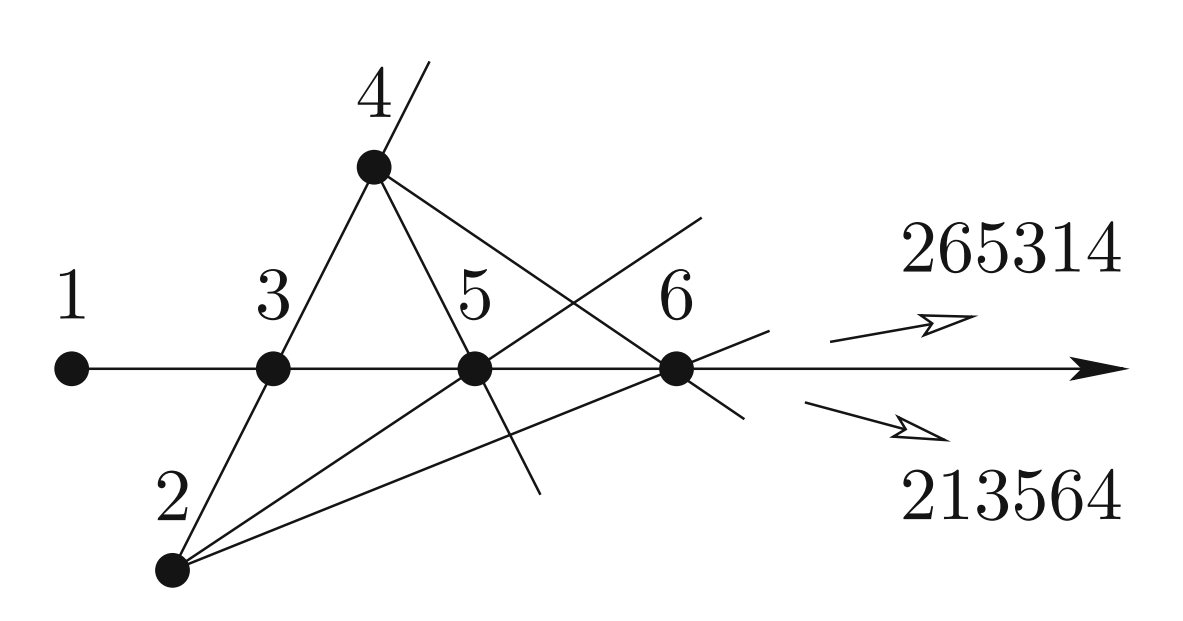
\includegraphics[scale=0.2]{pics/picture6.png}
    \caption{A crossing move}
\end{figure}

\noindent
\textbf{(4)} A \textit{touching move} is a move that reverses some string that is adjacent to the central barrier, but does not cross it. For example,

\begin{center}
$\pi_4 =$ 6\(\underline{25}\):3\(\underline{14}\) $\longrightarrow$ 6\(\overline{52}\):3\(\overline{41}\) $= \pi_5$
\end{center}

\noindent
is a touching move. Geometrically, a touching move corresponds to the slope of a line of the configuration that has exactly $m$ points on one side, and hence at most $m - 2$ points on the other side.

\noindent
Moves that are neither touching nor crossing will be called \textit{ordinary moves}. For this

\begin{center}
$\pi_1 =$ 213:5\(\underline{46}\) $\longrightarrow$ 213:5\(\overline{64}\) $= \pi_2$
\end{center}

\noindent
is an example. So every move is either crossing, or touching, or ordinary, and we can use the letters $T, C, O$ to denote the types of moves. $C(d)$ will denote a crossing move of order $d$. Thus for our small example we get

\[\pi_0 \overset{T}{\longrightarrow} \pi_1 \overset{O}{\longrightarrow} \pi_2 \overset{C(2)}{\longrightarrow} \pi_3 \overset{O}{\longrightarrow} \pi_4 \overset{T}{\longrightarrow} \pi_5 \overset{C(1)}{\longrightarrow} \pi_6,\]               

\noindent
or even shorter we can record this sequence as $T, O, C(2), O, T, C(1)$.

\begin{figure}[H]
    \centering
    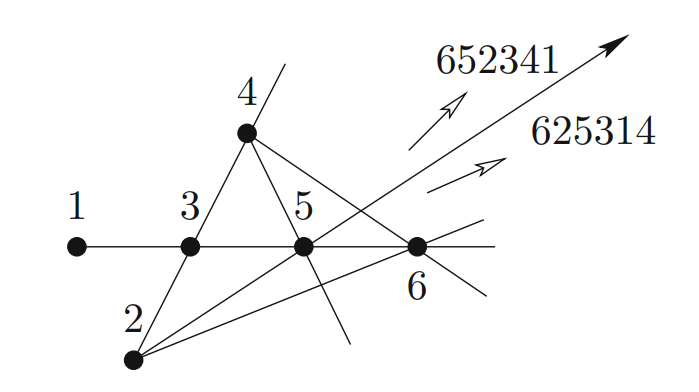
\includegraphics[scale=0.4]{pics/picture7.png}
    \caption{A touching move}
\end{figure}

\begin{figure}[H]
    \centering
    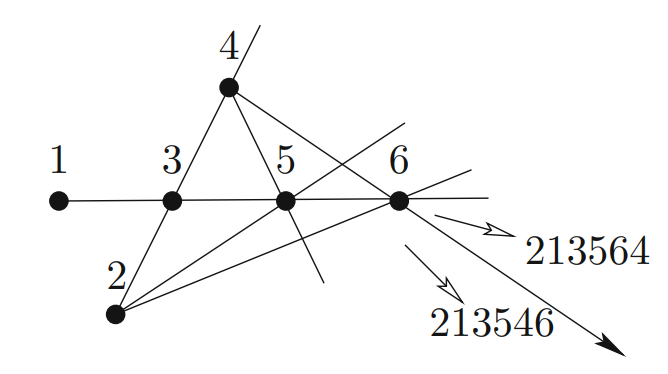
\includegraphics[scale=0.4]{pics/picture8.png}
    \caption{An ordinary move}
\end{figure}

\noindent
\textbf{(5)} To complete the proof, we need the following two facts:

\begin{itemize}
\item[ ]\textit{Between any two crossing moves, there is at least one touching move.}
\item[ ]\textit{Between any crossing move of order $d$ and the next touching move, there are at least $d - 1$ ordinary moves.}
\end{itemize}

\noindent
In fact, after a crossing move of order $d$ the barrier is contained in a symmetric decreasing substring of length $2d$, with $d$ letters on each side of the barrier. For the next crossing move the central barrier must be brought into an increasing substring of length at least $2$. But only touching moves affect whether the barrier is in an increasing substring. This yields the first fact. For the second fact, note that with each ordinary move (reversing some \textit{increasing} substrings) the decreasing $2d$-string can get shortened by only one letter on each side. And, as long as the decreasing string has at least 4 letters, a touching move is impossible. This yields the second fact.

\noindent
If we construct the sequence of permutations starting with the same initial projection but using a clockwise rotation, then we obtain the reversed sequence of permutations. Thus the sequence that we do have recorded must also satisfy the opposite of our second fact:

\begin{itemize}
\item[ ]\textit{Between a touching move and the next crossing move, of order $d$, there are at least $d − 1$ ordinary moves.}
\end{itemize}

\noindent
\textbf{(6)} The \textit{T-O-C}-pattern of the infinite sequence of permutations, as derived in (2), is obtained by repeating over and over again the \textit{T-O-C}-pattern of length $t$ of the sequence $\pi_0 \rightarrow \ldots \rightarrow \pi_t$. Thus with the facts of (5) we see that in the infinite sequence of moves, each crossing move of order $d$ is embedded into a \textit{T-O-C}-pattern of the type


$$
T,\underbrace{O, O, \ldots, O}_{\text{$\geq$ d−1}}  ,C(d),\underbrace{O, O, \ldots, O}_{\text{$\geq$ d−1}} \qquad (\ast)
$$


\noindent
of length $1+(d - 1) + 1 + (d - 1) = 2d$.
 
\noindent
In the infinite sequence, we may consider a finite segment of length $t$ that starts with a touching move. This segment consists of substrings of the type (∗), plus possibly extra inserted $T’$s. This implies that its length $t$ satisfies

\begin{center}
$ t \geq \sum_{i=1}^{c} 2d_i \geq n,$
\end{center}

\noindent
which completes the proof.

\end{proof}

% References
\bibliographystyle{plain}
\bibliography{mybib}

\end{document} 